%% \documentclass[a4paper]{article}
%% \usepackage{pgfplots}
%% \pgfplotsset{compat=1.16}
%% \begin{document}

\begin{tikzpicture}
\begin{semilogxaxis}[
  % title = Experiment on the time taken to find a bug,
  ylabel = Time (ms),
  xlabel = Invocations per thread,
  % ymax = 4,
  log basis x=2,
  scaled ticks = false,
  legend pos = north west,
  height = 0.4\textheight,
  width = 0.9\textwidth
]
\addplot+[error bars/.cd, y dir=both,y explicit] coordinates {
  (2,5871.77268287) +- (0,1241.652477706246)
  (4,744.931896425) +- (0,100.39702970192621)
  (8,932.286987545) +- (0,70.12118940035633)
  (16,1720.175756855) +- (0,299.7126481558856)
  (32,7054.778178755) +- (0,1090.8275119367097)
};
\addlegendentry{$p = 6$}
\addplot+[error bars/.cd, y dir=both,y explicit] coordinates {
  (2,2520.7805230999998) +- (0,436.88469830610507)
  (4,597.17587284) +- (0,60.12000519551778)
  (8,919.645957005) +- (0,150.83043713605863)
  (16,2269.57868647) +- (0,581.7104196004394)
  (32,5708.43440495) +- (0,1200.6556623094984)
};
\addlegendentry{$p = 9$}
\addplot+[error bars/.cd, y dir=both,y explicit] coordinates {
  (2,1888.5533899949999) +- (0,313.1773325056869)
  (4,548.37487376) +- (0,45.49308970263773)
  (8,1341.05564978) +- (0,294.92064545884415)
  (16,2252.633057365) +- (0,528.5362208882167)
  (32,6017.146730475) +- (0,1608.0484982668079)
};
\addlegendentry{$p = 15$}
\addplot+[error bars/.cd, y dir=both,y explicit] coordinates {
  (2,2340.958584985) +- (0,411.33241458373817)
  (4,804.12604088) +- (0,66.597760022275)
  (8,4314.4595586450005) +- (0,760.2132377988916)
  (16,7550.615771770001) +- (0,1217.5932232364776)
};
\addlegendentry{$p = 24$}
\end{semilogxaxis}
\end{tikzpicture}

% --samples 200 --tester ABCTester --maxItersPerRun 480
%% \end{document}
